% DOC SETTINGS ===================================
\documentclass{article}
\usepackage[utf8]{inputenc}
\usepackage{steinmetz}
\usepackage{mathtools}  
\usepackage{multicol}
\usepackage{circuitikz}
\usepackage{tikz}
\usepackage{listings}
\usepackage{geometry}
\usepackage{fancyhdr}
\usepackage{amsfonts}
\usepackage{media9}
\usepackage{parskip}
\usetikzlibrary{positioning, fit, calc}
\pagestyle{fancy}
\lhead{ECE2714 Problem Set 10}
\rhead{Kavin Thirukonda 2021}
\fancyheadoffset{0mm}
 \geometry{
 a4paper,
 total={170mm,257mm},
 left=20mm,
 top=25mm,
 }
\mathtoolsset{showonlyrefs} 
\cfoot{}
% DOC SETTINGS ===================================
\begin{document}
\begin{enumerate}
    \item Determine if the CT LTI system described by the LCCDE
    \begin{equation}
        \frac{d^3}{dt^3}y(t)-9\frac{d^2}{d^2}y(t) + 24\frac{d}{dt}y(t)+34y(t) = \frac{dx}{dt} +2x(t)
    \end{equation}
    is stable. Explain your rationale.
    \begin{align}
        &\frac{d^3}{dt^3}y(t)-9\frac{d^2}{d^2}y(t) + 24\frac{d}{dt}y(t)+34y(t) = 0\\
        &\Rightarrow D^3y(t)-9D^2y(t) + 24Dy(t)+34y(t) = 0\\
        &\Rightarrow (D^3-9D^2 + 24D+34)y(t) = 0\\
        &\Rightarrow (D + 1)(D^2-10D + 34)y(t) = 0\\
        &\Rightarrow D = -1 + 0j, 5-3j, 5+3j
    \end{align}
    \begin{center}
        This system is \boxed{\textbf{not stable}} as the real portion of all the roots are not negative, only one of them are.
    \end{center}
    \newpage
    \item Given a stable LTI system described by the LCCDE
    \begin{equation}
        \frac{d^3}{dt^3}y(t)+106\frac{d^2}{d^2}y(t) + 605\frac{d}{dt}y(t)+500y(t) = 100\frac{d}{dt}x(t) +200x(t)
    \end{equation}
    \begin{enumerate}
        \item Find the frequency response of the system
        \begin{align}
            &\frac{d^3}{dt^3}y(t)+106\frac{d^2}{d^2}y(t) + 605\frac{d}{dt}y(t)+500y(t) = 0\\
            &\Rightarrow D^3y(t)+106D^2y(t) + 605y(t)+500y(t) = 0\\
            &\Rightarrow (D^3+106D^2 + 605+500)y(t) = 0\\
            &\Rightarrow D = -100, -5, -1
        \end{align}
        \begin{align}
            &y_h(t) = C_1e^{-100t}+C_2e^{-5t}+C_3e^{-t}\big|_{y_h(0)=1}\\
            &y^{'}_h(t) = C_1e^{-100t}+C_2e^{-5t}+C_3e^{-t}\big|_{y^{'}_h(0)=0}\\
            &y^{''}_h(t) = C_1e^{-100t}+C_2e^{-5t}+C_3e^{-t}\big|_{y^{''}_h(0)=0}\\
            &\Rightarrow 1 = C_1+C_2+C_3\\
            &\Rightarrow 0 = -100C_1-5C_2-C_3\\
            &\Rightarrow 0 = 10000C_1+25C_2+C_3
        \end{align}
        \begin{equation}
            y_h(t) = \frac{1}{1881}e^{-100t}-\frac{5}{19}e^{-5t}+\frac{125}{99}e^{-t}
        \end{equation}
        \begin{align}
            h(t) &= (100D+200)(\frac{1}{1881}e^{-100t}-\frac{5}{19}e^{-5t}+\frac{125}{99}e^{-t})u(t)\\
            &= (-\frac{10000}{1881}e^{-100t}+\frac{2500}{76}e^{-5t}-\frac{12500}{396}e^{-t}+\frac{200}{1881}e^{-100t}-\frac{1000}{76}e^{-5t}+\frac{25000}{396}e^{-t})u(t)\\
            &= (-\frac{9800}{1881}e^{-100t}+\frac{1500}{76}e^{-5t}+\frac{12500}{396}e^{-t})u(t)
        \end{align}
        \begin{align}
            H(j\omega) &= \int_{-\infty}^\infty h(t)e^{-j\omega t}dt\\
            &= \int_{-\infty}^\infty (-\frac{9800}{1881}e^{-100t}+\frac{1500}{76}e^{-5t}+\frac{12500}{396}e^{-t})u(t)e^{-j\omega t}dt\\
            &= \int_{0}^\infty (-\frac{9800}{1881}e^{-100t}+\frac{1500}{76}e^{-5t}+\frac{12500}{396}e^{-t})e^{-j\omega t}dt\\
            &= \boxed{-\frac{9800}{1881(-100-j\omega)}+\frac{1500}{76(-5-j\omega)}+\frac{12500}{396(-1-j\omega)}}
            \end{align}
        \item If the input to this system is x(t) = cos(t), what is the output in the time domain, y(t)?
        \begin{align}
            y(t) = &\mathcal{F}\bigg\{\pi(-\frac{9800}{1881(-100-j\omega)}+\frac{1500}{76(-5-j\omega)}+\frac{12500}{396(-1-j\omega)})(\delta(\omega-1)+\delta(\omega+1))\bigg\}\\
            = &\pi\bigg(-\frac{9800}{1881(-100-j(\omega-1))}+\frac{1500}{76(-5-j(\omega-1))}+\frac{12500}{396(-1-j(\omega-1))}\\
            &-\frac{9800}{1881(-100-j(\omega+1))}+\frac{1500}{76(-5-j(\omega+1))}+\frac{12500}{396(-1-j(\omega+1))}\bigg)
        \end{align}
    \end{enumerate}
    \newpage
    \item Given the Bode plot for a system as follows
    \begin{center}
        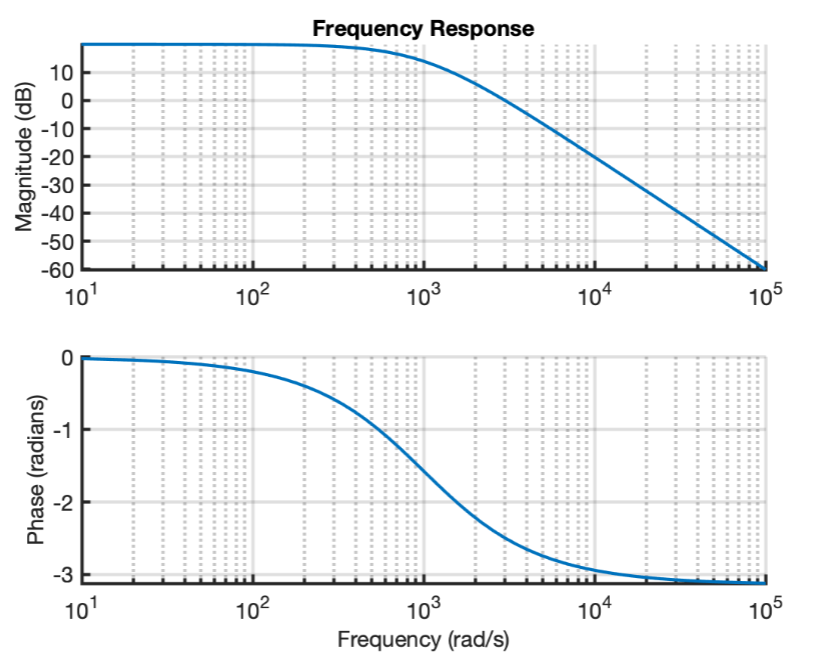
\includegraphics[width = .65\textwidth]{bode.png}
    \end{center}
    \begin{enumerate}
        \item What is the output if the input is $x(t) = e^{j100t}$?
        \begin{equation}
            e^{j100t} \mapsto 100e^{j99.75t}
        \end{equation}
        \item What is the output if the input is $x(t) = \sin(3000t)$
        \begin{equation}
            \sin(3000t) \mapsto 31.623\sin(3000t-2.5)
        \end{equation}
        \item What is the output if the input is $x(t) = \cos(10000t - \frac{\pi}{100})$?
        \begin{equation}
            \sin(10000t - \frac{\pi}{100}) \mapsto \frac{1}{100}\sin(10000t- \frac{\pi-300}{100})
        \end{equation}
    \end{enumerate}
    \newpage
    \item The output y(t) of a causal LTI system is related to the input x(t) by the differential equation   
    \begin{equation}
        \frac{d}{dt}y(t) + 2y(t) = x(t).
    \end{equation}
    The input x(t) to the system is given as
    \begin{equation}
        x(t) = e^{-t}u(t).
    \end{equation}
    Determine the Fourier tranform of the output, $Y(j\omega)$.
    \begin{equation}
        X(j\omega) = \frac{1}{1+j\omega}
    \end{equation}
    \begin{align}
        &\frac{d}{dt}y(t) + 2y(t) = x(t)\\
        &\Rightarrow D^1y(t) + 2y(t) = 0\\
        &\Rightarrow (D^1 + 2)y(t) = 0\\
        &\Rightarrow D = -2
    \end{align}
    \begin{equation}
        h(t) = e^{-2t}u(t)
    \end{equation}
    \begin{equation}
        H(j\omega) = \frac{1}{2+j\omega}
    \end{equation}
    \begin{equation}
        \boxed {Y(j\omega) = \frac{1}{(2+j\omega)(1+j\omega)}}
    \end{equation}
    \newpage
    \item Consider the following second-order  difference equation
    \begin{equation}
        y[n] + y[n-1] +\frac{1}{4}y[n-2] = x[n]
    \end{equation}
    Decide whether or not the step response is oscillatory and explain your reasoning.
    \begin{center}
        \textbf{Yes, It is oscillatory}. It is an oscillatory function with a decaying magnitudes, which is still oscillatory this can be seen by taking the roots of the characteristic equation and checking what they are in relation to zero.
    \end{center}
    \newpage
    \item Consider a discrete time system that produces output
    \begin{equation}
        y[n] = n\left(\frac{4}{5}\right)^nu[n]
    \end{equation}
    when the input is
    \begin{equation}
        x[n] = \left(\frac{4}{5}\right)^nu[n]
    \end{equation}
    \begin{enumerate}
        \item Determine the system frequency response $H(e^{j\omega})$
        \begin{equation}
            Y(e^{j\omega} = \frac{\frac{4}{5}e^{-j\omega}}{(1-\frac{4}{5}e^{-j\omega})^2}
        \end{equation}
        \begin{equation}
            X(e^{j\omega} = \frac{1}{(1-\frac{4}{5}e^{-j\omega})}
        \end{equation}
        \begin{equation}
            H(e^{j\omega} = \frac{\frac{4}{5}e^{-j\omega}}{1-\frac{4}{5}e^{-j\omega}}
        \end{equation}
        \item Determine the difference equation that defines the system
        \begin{equation}
            H(e^{j\omega}) = \frac{\frac{4}{5}e^{-j\omega}}{1-\frac{4}{5}e^{-j\omega}}
        \end{equation}
        \begin{equation}
            y[n] - \frac{4}{5}y[n-1] = \frac{4}{5}x[n-1]
        \end{equation}
        \item Determine the system impulse response
        \begin{equation}
            h[n] = \left(\frac{4}{5}\right)^nu[n-1]
        \end{equation}
    \end{enumerate}
\end{enumerate}
\end{document}
